\documentclass{natourDoc}
\usepackage{lipsum}
\usepackage{tabularx}
%\usepackage[table]{xcolor}
\usepackage{multirow}
\usepackage{svg}
\usepackage{amsmath}
\usepackage{pdfpages}
%\usepackage{placeins}
%\usepackage[T1]{fontenc}
\usepackage{ltablex}
\usepackage{longtable}
%\usepackage{hyperref}

\hypersetup{
    colorlinks=true,
    linkcolor=black,
    filecolor=magenta,
    urlcolor=blue,
}

%\newcolumntype{a}{>{\columncolor{PineGreen!70}}l}

\def\arraystretch{1.5}

\title{Documentazione IngSW} %Titolo

\begin{document}

%----------- Informazioni --------------------

\titolo{Specifica, progettazione, implementazione e validazione del Sistema Informativo\\ \textit{NaTour21}} %Titolo.pdf
\sottotitolo{Dipartimento di Ingegneria Elettrica \\ e delle Tecnologie dell'Informazione} %Nome progetto

\professors{Sergio    \textsc{Di Martino} \\
	Francesco \textsc{Cutugno}
} %Nome docenti

\students{Bianca Giada \textsc{Chehade} N86003209 \\
	Mario 	   \textsc{Liguori} N86003258 \\
	Mattia 	   \textsc{Rossi} 	N86003211
} %Nome studenti

%----------- Inizializzazione -----------------

\marginscreate %Crea margini
\cover %Crea cover
\toc %Crea Table of Contents

%------------ Corpo del documento ----------------

\section{Descrizione del progetto}
NaTour21 è un sistema complesso e distribuito finalizzato ad offrire un moderno social network multipiattaforma per appassionati di escursioni.\\

Il sistema consiste in:
\begin{itemize}
	\item un Back-End sicuro, performante e scalabile;
	\item un client mobile attraverso cui gli
	      utenti possono fruire delle funzionalità del sistema in modo intuitivo, rapido e piacevole;
	\item un client mobile attraverso cui gli amministratori possono gestire i contenuti inseriti in piattaforma.\\
\end{itemize}

NaTour21 ha lo scopo di creare una community sicura e affidabile dove condividere la propria passione per l'escursionismo.\\

In questo scenario, l'utente si configura come protagonista: oltre alla possibilità di inserire itinerari (dettagliati da informazioni), compilation e post personali sulla piattaforma,
è lasciato ampio spazio all'individualità personale.\\

Tutto ciò si concretizza con la possibilità di interagire con gli altri utenti, in modo da poter avere un contatto più diretto con
la realtà dell'escursionismo, e di lasciare valutazioni personali su qualunque itinerario si desideri.\\

Il sistema valuta essenziale la sicurezza degli utenti: questi potranno segnalare informazioni inesatte o contenuti inappropriati al fine
di rendere la permanenza nella community piacevole per tutti.

\subsection{Presentazione dell'idea progettuale}

L'applicazione "NaTour21" nasce in seguito all'esigenza di uno spazio virtuale dove poter condividere la passione per l'escursionismo.\\
Creare una community di escursionisti, esperti o meno, ha lo scopo di rendere le esperienze individuali degli utenti più sicure e informate,
oltre a promuovere la condivisione di contenuti personali.\\\\
NaTour21 mette a disposizione degli utenti registrati diverse funzionalità.\\
Il lato prettamente informativo consente di ricercare - nonchè inserire in piattaforma - diversi itinerari, e tutte le informazioni relative ad essi.
Ciò comprende la possibilità di visualizzarli su mappa, e, per garantire un'accuratezza maggiore delle informazioni, di lasciare
un feedback personale per ciascuno di essi.\\\\
Ci sono, però, ulteriori funzionalità che coinvolgono direttamente l'utente: tra queste la condivisione di post, la creazione di compilation personalizzate e
la visualizzazione di una homepage con post riguardanti diversi itinerari.\\
Particolare attenzione è riservata alla sicurezza degli utenti, i quali possono segnalare contenuti inappropriati o informazioni inesatte.

\subsection{Individuazione del target degli utenti}
NaTour21 si configura come community in cui chiunque può intraprendere la passione per l'escursionismo e condividerla.\\\\
Ciononostante, è stato possibile individuare un target di utenti ben definito grazie ai dati
statistici\footnote{Fonte: \href{http://dati.istat.it/Index.aspx?DataSetCode=DCCV_ESC_CAPI}{sito ufficiale Istat}.} raccolti
nell'anno 2020 dall'ISTAT, Istituto Nazionale di Statistica.\\\\
In seguito all'analisi delle informazioni statistiche sull'escursionismo italiano è stato individuato come target utenti la popolazione, caratterizzata da un
numero di circa pari entità di uomini e di donne, nella fascia di età \texttt{35-64}. La maggior parte della
platea considerata risulta essere appartenente alla condizione lavorativa di \textit{dirigente, quadro o impiegato}.\\\\
\begin{figure}[!htbp]
	\centering
	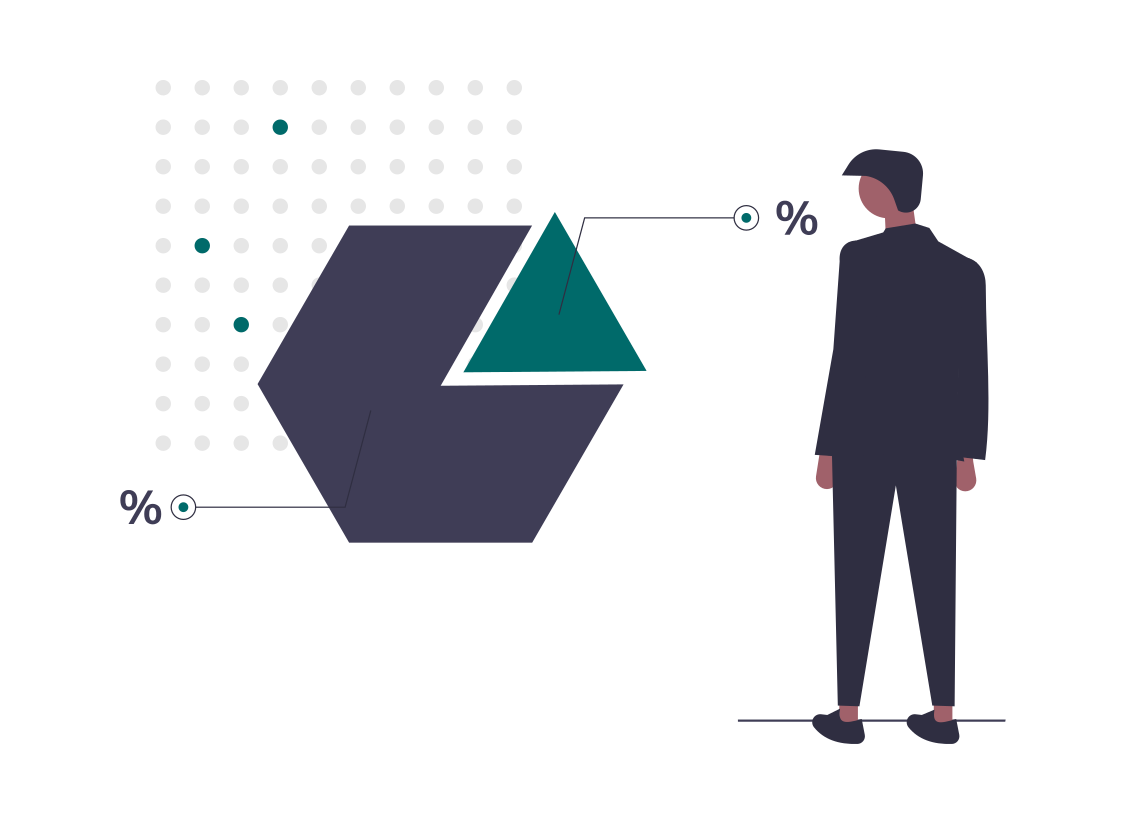
\includegraphics[width=12cm, page=1]{./logos/undraw_statistic_chart_38b6.png}
\end{figure}
\FloatBarrier
L'Istat ha inoltre conteggiato nell'anno 2020 circa \texttt{41194} escursioni giornaliere,
di cui il \texttt{42.7\%} situate temporalmente nel terzo trimestre dell'anno. Da questa informazione si deduce che il periodo
preferito per attività escursionistiche sia quello dei mesi estivi.\\\\
Il motivo prevalente per queste escursioni risulta essere stato \textit{piacere personale, svago e tempo libero}, con un numero
di escursioni così orientate pari a \texttt{23223}: questo dato risulta particolarmente significativo, pari a un ordine
di grandezza in più rispetto agli altri motivi registrati. È importante anche notare quanto il numero di escursioni in paesi
esteri sia di gran lunga minore rispetto a quelle nelle regioni italiane.\\\\
Le regioni del Nord Italia sembrano essere state le preferite per visite giornaliere (la più visitata è stata il Veneto, con una media di
\texttt{6200}), seguite immediatamente da quelle del centro-Sud. Il Molise, invece, non risulta aver raggiunto
la minima cifra considerata nella raccolta dati.\\

\subsection{Valutazione dell'usabilità a priori}

\subsubsection{Contesto d’uso del prodotto}
La nostra applicazione NaTour sarà utilizzabili grazie ad una connessione 
internet e GPS, poiché tale app porta l’utente in luoghi distanti dal contesto 
urbano dovrà fare affidamento sulla propria connessione. 
Il contesto immaginato per l’utilizzo della nostra applicazione è dare la possibilità ad appassionati di escursionismo di poter accedere in 
modo semplice e intuitivo ad un’applicazione che contenga itinerari creati e valutati da altri utenti, 
oppure essere noi i creatori di tali percorsi che verranno poi usufruiti da altri utenti. 
Invece di impiegare tempo a ricercare itinerari con cui si potrebbe persino non aver un riscontro, 
basta una semplice ricerca sulla nostra applicazione per trovare itinerari non solo vicini all’utente, 
ma anche aver la possibilità di creare dei post per tali itinerari, 
in modo da ottenere un riscontro con altri utenti, 
oppure di creare compilation di itinerari da avere sempre a disposizione.

\subsubsection{Valutazione dell’usabilità}
Parte fondamentale nel processo creativo dell’applicazione è sempre capire in che direzione andare per migliorare l’esperienza dei clienti. Per realizzare ciò siamo ricorsi ad alcune tecniche per testare l’usabilità del nostro prodotto. L’approccio da noi adottato richiede di far eseguire dei task a un gruppo di utenti con differenti retroscena. Tali task vengono approcciati con due possibili: 
	L’utente è stato in grado di compiere il task tramite gli strumenti offertigli dall’app.
	L’utente non è stato in grado di compiere il task tramite gli strumenti offertigli dall’app.
Ciò naturalmente deve essere eseguito in maniera completamente autonoma dall’utente senza uscire dall’app. 


\newpage
\subsection{Definizione delle personas}
\begin{figure}[!htbp]
	\centering
	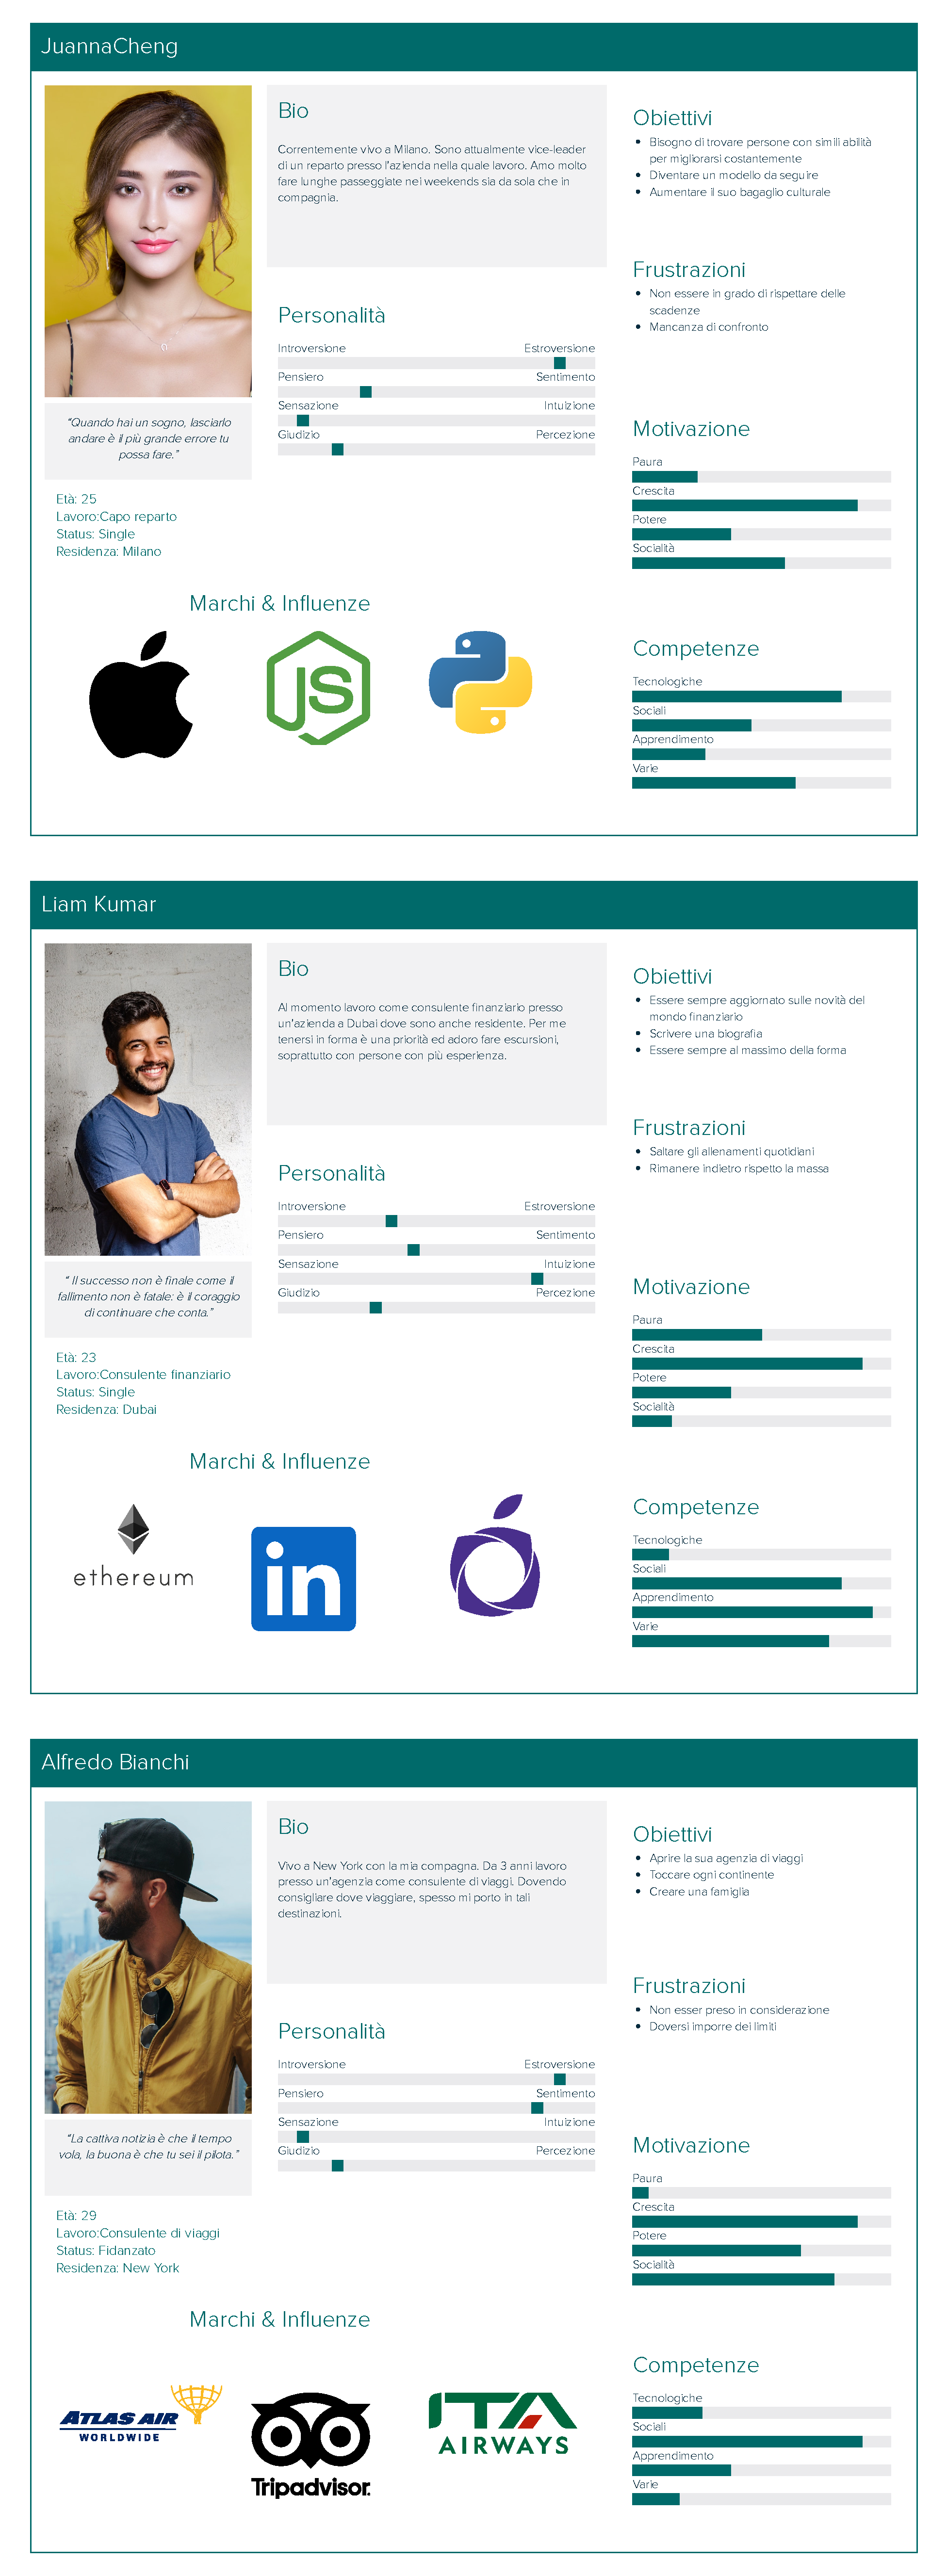
\includegraphics[width=\textwidth, page=1]{./personas/Personas.pdf}
\end{figure}
\FloatBarrier

\section{Documento dei Requisiti Software}
\subsection{Requisiti funzionali}
In questa sezione saranno esposti i requisiti \textit{funzionali} dell'applicazione NaTour21, cioè le funzionalità richieste dai commissionanti.

\subsubsection{Autenticazione}
\begin{table}[H]
	\centering
	\begin{tabular}{ |p{5cm}|p{10.3cm}| }
		\hline
		\rowcolor{PineGreen!70}
		\textbf{Nome} & \textbf{Descrizione}                                                                                                                                      \\
		\hline
		Registrazione & Il sistema deve consentire ad un utente di potersi registrare indicando e-mail e password, oppure utilizzando account di terze parti (Google o Facebook). \\
		\hline
	\end{tabular}
	\caption{RF.1}
	\label{table:1}
\end{table}

\begin{table}[H]
	\centering
	\begin{tabular}{ |p{5cm}|p{10.3cm}| }
		\hline
		\rowcolor{PineGreen!70}
		\textbf{Nome} & \textbf{Descrizione}                                                                    \\
		\hline
		Accesso & Il sistema deve consentire ad un utente di poter effettuare l'accesso alla piattaforma avente eseguito precendentemente una registrazione. \\
		\hline
	\end{tabular}
	\caption{RF.2}
	\label{table:2}
\end{table}

\begin{table}[H]
	\centering
	\begin{tabular}{ |p{5cm}|p{10.3cm}| }
		\hline
		\rowcolor{PineGreen!70}
		\textbf{Nome} & \textbf{Descrizione}                                                                                             \\
		\hline
		Reimpostazione password & Il sistema deve consentire ad un utente registrato di poter cambiare la propria password se dimenticata o persa. \\
		\hline
	\end{tabular}
	\caption{RF.3}
	\label{table:3}
\end{table}

\begin{table}[H]
	\centering
	\begin{tabular}{ |p{5cm}|p{10.3cm}| }
		\hline
		\rowcolor{PineGreen!70}
		\textbf{Nome} & \textbf{Descrizione}                                                                                             \\
		\hline
		Uscita dall'account & Il sistema deve consentire ad un utente registrato di poter uscire dal'account con il quale ha eseguito l'accesso. \\
		\hline
	\end{tabular}
	\caption{RF.3}
	\label{table:3}
\end{table}


\subsubsection{Interazione con un itinerario}
\begin{table}[H]
	\centering
	\begin{tabular}{ |p{5cm}|p{10.3cm}| }
		\hline
		\rowcolor{PineGreen!70}
		\textbf{Nome}             & \textbf{Descrizione}                                                 \\
		\hline
		Visualizzazione itinerari & Il sistema deve consentire a un utente autenticato di visualizzare i
		dettagli degli itinerari pubblicati e i post ad essi associati.                                  \\
		\hline
	\end{tabular}
	\caption{RF.4}
	\label{table:4}
\end{table}

\begin{table}[H]
	\centering
	\begin{tabular}{ |p{5cm}|p{10.3cm}| }
		\hline
		\rowcolor{PineGreen!70}
		\textbf{Nome}          & \textbf{Descrizione}                                                                                                    \\
		\hline
		Inserimento itinerario & Il sistema deve consentire a un utente autenticato di inserire nuovi itinerari (sentieri) in piattaforma. Un sentiero è
		caratterizzato da un nome, una durata (max 16 ore), un livello di difficoltà, un punto di inizio e di fine, delle foto (max 5), una descrizione
		(opzionale), e un tracciato geografico (opzionale) che lo rappresenta su una mappa. Il tracciato
		geografico può essere inseribile manualmente (interagendo con una mappa interattiva) oppure
		tramite file in formato standard GPX.                                                                                                            \\
		\hline
	\end{tabular}
	\caption{RF.5}
	\label{table:5}
\end{table}

\begin{table}[H]
	\centering
	\begin{tabular}{ |p{5cm}|p{10.3cm}| }
		\hline
		\rowcolor{PineGreen!70}
		\textbf{Nome}     & \textbf{Descrizione}                                                                                                                                               \\
		\hline
		Ricerca itinerari & Il sistema deve consentire a un utente autenticato di effettuare ricerche di itinerari tra quelli presenti in piattaforma, con possibilità di filtrare i risultati
		per area geografica, per livello di difficoltà, per durata e per accessibilità ai disabili.                                                                                           \\
		\hline
	\end{tabular}
	\caption{RF.6}
	\label{table:6}
\end{table}

\begin{table}[H]
	\centering
	\begin{tabular}{ |p{5cm}|p{10.3cm}| }
		\hline
		\rowcolor{PineGreen!70}
		\textbf{Nome}          & \textbf{Descrizione}                                                                                   \\
		\hline
		Valutazione itinerario & Il sistema deve consentire a un utente autenticato di indicare un punteggio di difficoltà e/o un tempo
		di percorrenza diverso da quello indicato dall’utente che ha inserito il sentiero. In questo caso, il
		punteggio di difficoltà e il tempo di percorrenza per il sentiero saranno ri-calcolati come la media
		delle difficoltà e dei tempi indicati.                                                                                            \\
		\hline
	\end{tabular}
	\caption{RF.7}
	\label{table:7}
\end{table}

\begin{table}[H]
	\centering
	\begin{tabular}{ |p{5cm}|p{10.3cm}| }
		\hline
		\rowcolor{PineGreen!70}
		\textbf{Nome}          & \textbf{Descrizione}                                                        \\
		\hline
		Salvataggio itinerario & Il sistema deve consentire a un utente autenticato di salvare gli itinerari
		nelle proprie compilation personalizzate.                                                            \\
		\hline
	\end{tabular}
	\caption{RF.8}
	\label{table:8}
\end{table}

\begin{table}[H]
	\centering
	\begin{tabular}{ |p{5cm}|p{10.3cm}| }
		\hline
		\rowcolor{PineGreen!70}
		\textbf{Nome}           & \textbf{Descrizione}                                                            \\
		\hline
		Segnalazione itinerario & Il sistema deve consentire a un utente autenticato di segnalare degli itinerari
		le quali informazioni potrebbero non essere corrette e/o aggiornate.                                      \\
		\hline
	\end{tabular}
	\caption{RF.9}
	\label{table:9}
\end{table}

\begin{table}[H]
	\centering
	\begin{tabular}{ |p{5cm}|p{10.3cm}| }
		\hline
		\rowcolor{PineGreen!70}
		\textbf{Nome}        & \textbf{Descrizione}                                                             \\
		\hline
		Rimozione itinerario & Il sistema deve consentire a un utente autenticato di eliminare itinerari di cui
		è l'autore.                                                                                             \\
		\hline
	\end{tabular}
	\caption{RF.10}
	\label{table:10}
\end{table}

\subsubsection{Interazione con un post}
\begin{table}[H]
	\centering
	\begin{tabular}{ |p{5cm}|p{10.3cm}| }
		\hline
		\rowcolor{PineGreen!70}
		\textbf{Nome}        & \textbf{Descrizione}                                               \\
		\hline
		Visualizzazione post & Il sistema deve consentire a un utente autenticato di visualizzare
		i dettagli di un post.                                                                    \\
		\hline
	\end{tabular}
	\caption{RF.11}
	\label{table:11}
\end{table}

\begin{table}[H]
	\centering
	\begin{tabular}{ |p{5cm}|p{10.3cm}| }
		\hline
		\rowcolor{PineGreen!70}
		\textbf{Nome}    & \textbf{Descrizione}                                                    \\
		\hline
		Inserimento post & Il sistema deve consentire a un utente autenticato di inserire un post associato ad un itinerario,
		caratterizzato da foto (max 5) e una descrizione (opzionale).     \\
		\hline
	\end{tabular}
	\caption{RF.12}
	\label{table:12}
\end{table}


\begin{table}[H]
	\centering
	\begin{tabular}{ |p{5cm}|p{10.3cm}| }
		\hline
		\rowcolor{PineGreen!70}
		\textbf{Nome}     & \textbf{Descrizione}                                                                \\
		\hline
		Segnalazione post & Il sistema deve consentire a un utente autenticato di segnalare post con fotografie
		inappropriate.                                                                                          \\
		\hline
	\end{tabular}
	\caption{RF.13}
	\label{table:13}
\end{table}

\begin{table}[H]
	\centering
	\begin{tabular}{ |p{5cm}|p{10.3cm}| }
		\hline
		\rowcolor{PineGreen!70}
		\textbf{Nome}  & \textbf{Descrizione}                                                        \\
		\hline
		Rimozione post & Il sistema deve consentire a un utente autenticato di eliminare post di cui
		è l'autore.                                                                                  \\
		\hline
	\end{tabular}
	\caption{RF.14}
	\label{table:14}
\end{table}

\subsubsection{Gestione dati personali e conversazioni private}
\begin{table}[H]
	\centering
	\begin{tabular}{ |p{5cm}|p{10.3cm}| }
		\hline
		\rowcolor{PineGreen!70}
		\textbf{Nome}    & \textbf{Descrizione}                                                          \\
		\hline
		Gestione profilo & Il sistema deve consentire a un utente autenticato di gestire il suo profilo,
		egli potrà visitare i contenuti inseriti ed eliminarli. Inoltre potrà cambiare la foto profilo.  \\
		\hline
	\end{tabular}
	\caption{RF.15}
	\label{table:15}
\end{table}

\begin{table}[H]
	\centering
	\begin{tabular}{ |p{5cm}|p{10.3cm}| }
		\hline
		\rowcolor{PineGreen!70}
		\textbf{Nome}                  & \textbf{Descrizione}                                                                           \\
		\hline
		Gestione conversazioni private & Il sistema deve permettere all'utente autenticato lo scambio di informazioni con altri utenti.
		È possibile avviare la conversazione a partire dai contenuti pubblicati. Inoltre è possibile ricercare un destinatario.         \\
		\hline
	\end{tabular}
	\caption{RF.16}
	\label{table:16}
\end{table}

\subsubsection{Interazione con una compilation}
\begin{table}[H]
	\centering
	\begin{tabular}{ |p{5cm}|p{10.3cm}| }
		\hline
		\rowcolor{PineGreen!70}
		\textbf{Nome}         & \textbf{Descrizione}                                                                                    \\
		\hline
		Creazione compilation & Il sistema deve consentire a un utente autenticato di creare delle \textit{compilation personalizzate},
		caratterizzate da un titolo e da una descrizione.                                                                               \\
		\hline
	\end{tabular}
	\caption{RF.17}
	\label{table:17}
\end{table}

\begin{table}[H]
	\centering
	\begin{tabular}{ |p{5cm}|p{10.3cm}| }
		\hline
		\rowcolor{PineGreen!70}
		\textbf{Nome}         & \textbf{Descrizione}                                                       \\
		\hline
		Rimozione compilation & Il sistema deve consentire a un utente autenticato di eliminare le proprie
		compilation personalizzate                                                                         \\
		\hline
	\end{tabular}
	\caption{RF.18}
	\label{table:18}
\end{table}

\begin{table}[H]
	\centering
	\begin{tabular}{ |p{5cm}|p{10.3cm}| }
		\hline
		\rowcolor{PineGreen!70}
		\textbf{Nome}               & \textbf{Descrizione}                                                          \\
		\hline
		Visualizzazione compilation & Il sistema deve consentire a un utente autenticato di visualizzare i dettagli
		delle proprie compilation.                                                                                  \\
		\hline
	\end{tabular}
	\caption{RF.19}
	\label{table:19}
\end{table}


\begin{table}[H]
	\centering
	\begin{tabular}{ |p{5cm}|p{10.3cm}| }
		\hline
		\rowcolor{PineGreen!70}
		\textbf{Nome}                       & \textbf{Descrizione}                                                          \\
		\hline
		Rimozione itinerario da compilation & Il sistema deve consentire a un utente autenticato di eliminare gli itinerari
		che compongono le proprie compilation personalizzate                                                                \\
		\hline
	\end{tabular}
	\caption{RF.20}
	\label{table:20}
\end{table}

\subsubsection{Requisiti amministratore}
\begin{table}[H]
	\centering
	\begin{tabular}{ |p{5cm}|p{10.3cm}| }
		\hline
		\rowcolor{PineGreen!70}
		\textbf{Nome}                & \textbf{Descrizione}                                                                                \\
		\hline
		Visualizzazione segnalazioni & Il sistema deve permettere all'utente autenticato con i privilegi di amministratore di visualizzare
		la lista di segnalazioni inviate.                                                                                                  \\
		\hline
	\end{tabular}
	\caption{RF.21}
	\label{table:21}
\end{table}

\begin{table}[H]
	\centering
	\begin{tabular}{ |p{5cm}|p{10.3cm}| }
		\hline
		\rowcolor{PineGreen!70}
		\textbf{Nome}              & \textbf{Descrizione}                                                                                \\
		\hline
		Amministrazione itinerario & Il sistema deve permettere all'utente autenticato con i privilegi di amministratore di modificare o
		rimuovere un itinerario segnalato.                                                                                               \\
		\hline
	\end{tabular}
	\caption{RF.22}
	\label{table:22}
\end{table}

\subsection{Requisiti non funzionali}
Questa sezione conterrà invece i requisiti \textit{non funzionali} dell'applicazione, ovvero tutti i vincoli sui servizi offerti dal sistema.

\begin{table}[H]
	\centering
	\begin{tabular}{ |p{5cm}|p{10.3cm}| }
		\hline
		\rowcolor{PineGreen!70}
		\textbf{Nome}      & \textbf{Descrizione}                                                                 \\
		\hline
		Back-End scalabile & Il sistema deve essere scalabile e performante rispetto ai cambiamenti del Back-End,
		in modo da garantire un'agile manutenibilità nel tempo.                                                   \\
		\hline
	\end{tabular}
	\caption{RNF1}
	\label{table:23}
\end{table}

\begin{table}[H]
	\centering
	\begin{tabular}{ |p{5cm}|p{10.3cm}| }
		\hline
		\rowcolor{PineGreen!70}
		\textbf{Nome}      & \textbf{Descrizione}                                            \\
		\hline
		Sicurezza password & Il sistema non consente di inserire password che non contengano
		almeno 6 caratteri, di cui un carattere maiuscolo e un numero.                       \\
		\hline
	\end{tabular}
	\caption{RNF2}
	\label{table:24}
\end{table}


\begin{table}[H]
	\centering
	\begin{tabular}{ |p{5cm}|p{10.3cm}| }
		\hline
		\rowcolor{PineGreen!70}
		\textbf{Nome}                      & \textbf{Descrizione}                                       \\
		\hline
		Singola valutazione per itinerario & Il sistema non consente di inserire più di una valutazione
		per itinerario.                                                                                 \\
		\hline
	\end{tabular}
	\caption{RNF3}
	\label{table:25}
\end{table}

\begin{table}[H]
	\centering
	\begin{tabular}{ |p{5cm}|p{10.3cm}| }
		\hline
		\rowcolor{PineGreen!70}
		\textbf{Nome}                  & \textbf{Descrizione}                                                    \\
		\hline
		Segnalazione unica per un post & Il sistema non consente di inviare più di una segnalazione per un post. \\
		\hline
	\end{tabular}
	\caption{RNF4}
	\label{table:26}
\end{table}

\begin{table}[H]
	\centering
	\begin{tabular}{ |p{5cm}|p{10.3cm}| }
		\hline
		\rowcolor{PineGreen!70}
		\textbf{Nome}          & \textbf{Descrizione}                                                     \\
		\hline
		Numero massimo di foto & Il sistema non consente di inserire più di 5 foto per itinerario o post. \\
		\hline
	\end{tabular}
	\caption{RNF5}
	\label{table:27}
\end{table}

\newpage

\subsection{Requisiti di dominio}
Infine, questa sezione conterrà i requisiti \textit{di dominio} dell'applicazione, ovvero tutti i vincoli generali a cui l'applicativo
deve attenersi. \\

\begin{table}[H]
	\centering
	\begin{tabular}{ |p{5cm}|p{10.3cm}| }
		\hline
		\rowcolor{PineGreen!70}
		\textbf{Nome}      & \textbf{Descrizione}                                              \\
		\hline
		ISO/IEC 27018:2019 & Il sistema deve essere conforme allo standard ISO/IEC 27018:2019,
		incentrato sulla protezione dei dati personali nel cloud.                              \\
		\hline
	\end{tabular}
	\caption{RD1}
	\label{table:28}
\end{table}

\begin{table}[H]
	\centering
	\begin{tabular}{ |p{5cm}|p{10.3cm}| }
		\hline
		\rowcolor{PineGreen!70}
		\textbf{Nome} & \textbf{Descrizione}                                                                      \\
		\hline
		GDPR          & Il sistema deve essere conforme al GDPR (Regolamento Generale sulla Protezione dei Dati),
		incentrato sul trattamento dei dati personali e sulla privacy dell’utente.                                \\
		\hline
	\end{tabular}
	\caption{RD2}
	\label{table:29}
\end{table}

\newpage

\newpage
\subsection{Modellazione dei Casi d'Uso}
In questa sezione sarà riportato il diagramma Use Case per l'applicazione.\\
Per garantire una maggiore leggibilità e data la molteplicità di funzioni garantite
dal sistema, si è fatta la scelta di raggruppare le funzioni logicamente legate
tra loro in packages.

\begin{figure}[!htbp]
	\centering
	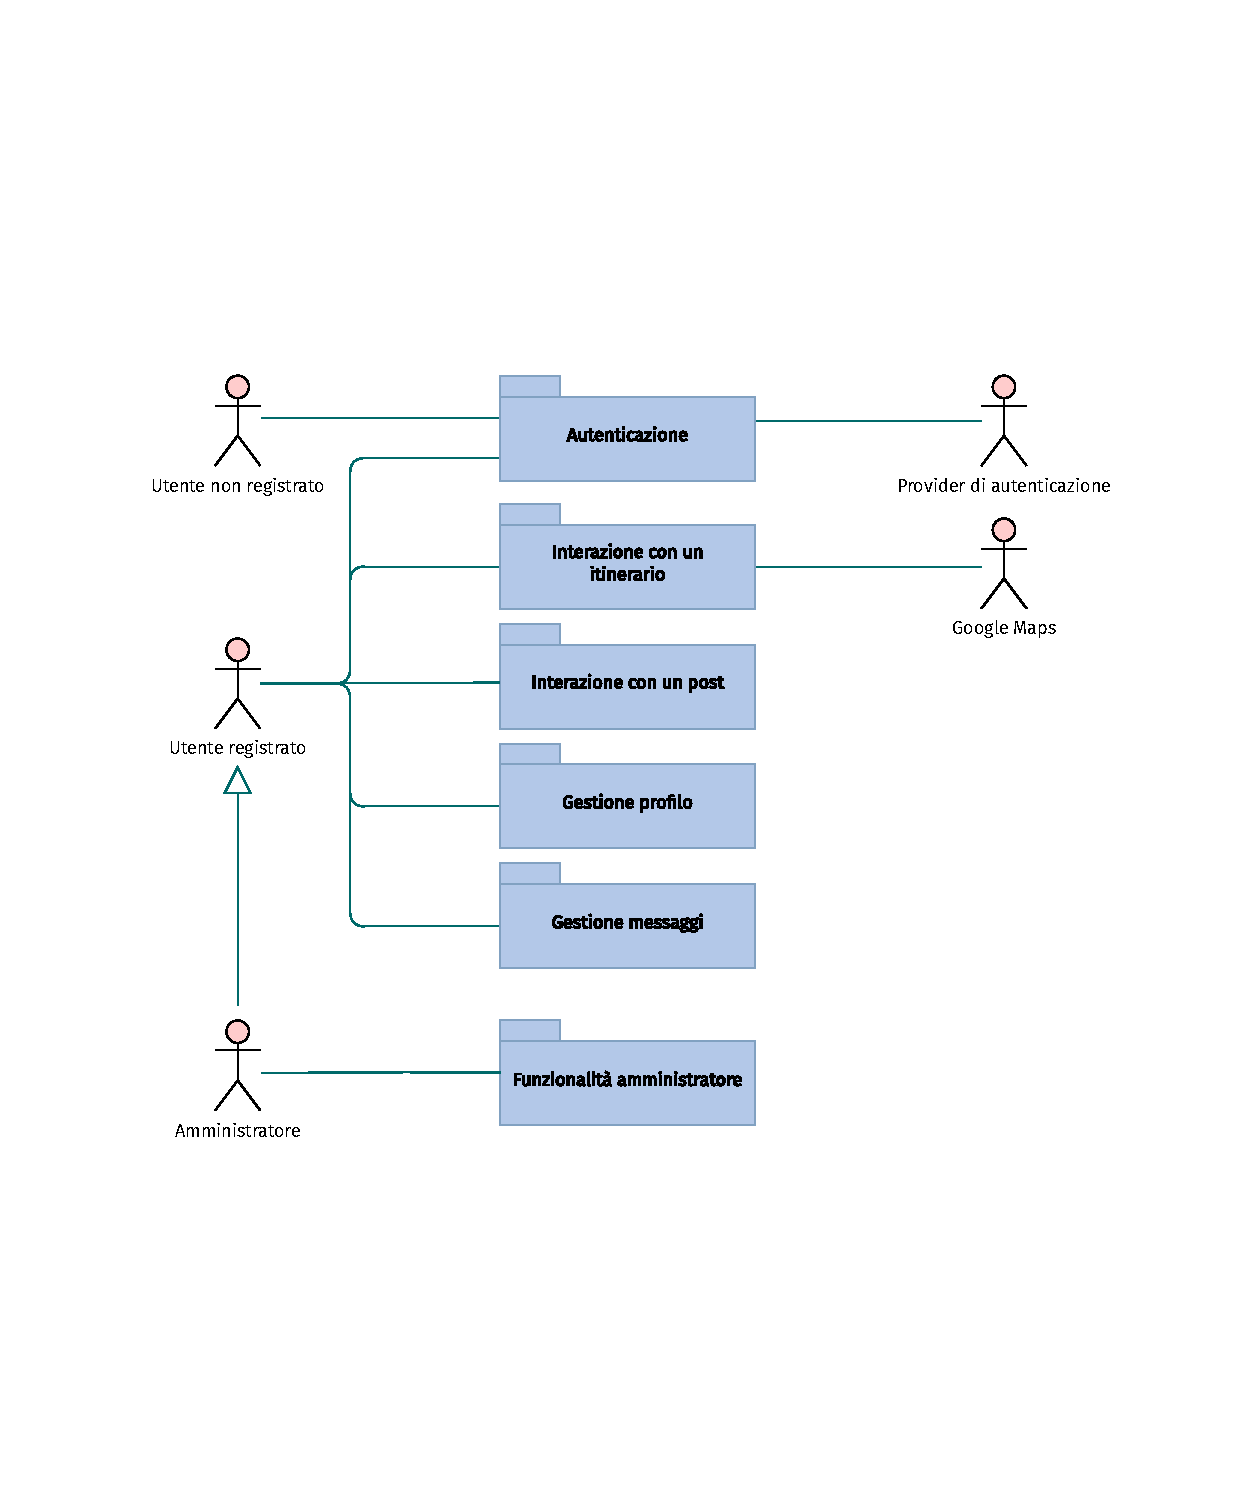
\includegraphics[width=\textwidth, page=1]{./diagrams/useCase.pdf}
	\caption{Use Case Diagram}
\end{figure}
\FloatBarrier

\newpage
\subsubsection{Autenticazione}
\begin{figure}[!htbp]
	\centering
	\includegraphics[width=\textwidth, page=2]{./diagrams/useCase.pdf}
	\caption{Package 1 - Autenticazione}
\end{figure}
\FloatBarrier

\newpage
\subsubsection{Interazione con un itinerario}
\begin{figure}[!htbp]
	\centering
	\includegraphics[width=\textwidth, page=3]{./diagrams/useCase.pdf}
	\caption{Package 2 - Interazione con un itinerario}
\end{figure}
\FloatBarrier

\newpage
\subsubsection{Interazione con un post}
\begin{figure}[!htbp]
	\centering
	\includegraphics[width=\textwidth, page=4]{./diagrams/useCase.pdf}
	\caption{Package 3 - Interazione con un post}
\end{figure}
\FloatBarrier

\newpage
\subsubsection{Gestione profilo}
\begin{figure}[!htbp]
	\centering
	\includegraphics[width=\textwidth, page=5]{./diagrams/useCase.pdf}
	\caption{Package 4 - Gestione profilo}
\end{figure}
\FloatBarrier

\newpage
\subsubsection{Gestione messaggi}
\begin{figure}[!htbp]
	\centering
	\includegraphics[width=\textwidth, page=6]{./diagrams/useCase.pdf}
	\caption{Package 5 - Gestione messaggi}
\end{figure}
\FloatBarrier

\newpage
\subsubsection{Funzionalità amministratore}
\begin{figure}[!htbp]
	\centering
	\includegraphics[width=\textwidth, page=7]{./diagrams/useCase.pdf}
	\caption{Package 6 - Funzionalità amministratore}
\end{figure}
\FloatBarrier

\newpage
\subsection{Tabelle di Cockburn dei casi d'uso}
Sono presentate in questa sezione le tabelle di Cockburn relative a due casi d'uso significativi dell'UCD.

\subsubsection{Inserisce un itinerario}

\def\arraystretch{1.5}
\begin{tabularx}{\linewidth}{| l | p{1cm} | p{4cm} | X | X|}
	\hline
	\textbf{USE CASE \#1}         & \multicolumn{4} {l|}{\textbf{Inserisce un itinerario}}                                                                                                                                                                                                                                                                                                                                                                                                      \\
	\hline Goal in Context        & \multicolumn{4}{>{\hsize=\dimexpr 4\hsize+4\tabcolsep+2\arrayrulewidth\relax}X|}{L’utente vuole inserire un itinerario in piattaforma}                                                                                                                                                                                                                                                                                                                      \\

	\hline Preconditions          &
	\multicolumn{4}{l|}{L’utente è autenticato}                                                                                                                                                                                                                                                                                                                                                                                                                                                 \\

	\hline Success End Conditions &
	\multicolumn{4}{l|}{L’utente riesce ad inserire il nuovo itinerario}                                                                                                                                                                                                                                                                                                                                                                                                                        \\

	\hline Failed End Conditions  &
	\multicolumn{4}{l|}{L’utente non riesce ad inserire il nuovo itinerario}                                                                                                                                                                                                                                                                                                                                                                                                                    \\

	\hline Primary Actor          &
	\multicolumn{4}{l|}{Utente registrato}                                                                                                                                                                                                                                                                                                                                                                                                                                                      \\

	\hline Secondary Actor        &
	\multicolumn{4}{l|}{Google Maps}                                                                                                                                                                                                                                                                                                                                                                                                                                                            \\

	\hline Trigger                & \multicolumn{4}{>{\hsize=\dimexpr 4\hsize+4\tabcolsep+2\arrayrulewidth\relax}X|}{                                                                                                                                                                                                                                                                                                                                                                           %
	L’utente preme il Floating Action Button “newRouteFab” nella schermata “RoutesUI”  }                                                                                                                                                                                                                                                                                                                                                                                                        \\

	\hline
	\multirow{2}{*}{}
	                              & Step                                                                                                                                   & Utente registrato                                                                                                                                                    & Sistema                                             & Google Maps                                                                           \\

	\cline{2-5}                   & 1                                                                                                                                      & Preme il Floating Action Button “newRouteFab” nella schermata “RoutesUI”
	                              &                                                                                                                                        &                                                                                                                                                                                                                                                                                                                    \\

	\cline{2-5}                   & 2                                                                                                                                      &                                                                                                                                                                      & Mostra la schermata “CreateRouteInfoUI”             &                                                                                       \\

	\cline{2-5}                   & 3                                                                                                                                      & Inserisce il nome dell’itinerario, (opzionalmente) la descrizione, la durata approssimativa, il livello di difficoltà e la possibilità di accessibilità per disabili &                                                     &                                                                                       \\

	\cline{2-5}                   & 4                                                                                                                                      & Preme il Floating Action Button “nextFab”                                                                                                                            &                                                     &                                                                                       \\

	\cline{2-5}                   & 5                                                                                                                                      &                                                                                                                                                                      & Mostra la schermata “NewRouteMapUI”                 &                                                                                       \\

	\cline{2-5}                   & 6                                                                                                                                      & Preme sull’icona di ricerca                                                                                                                                          &                                                     &                                                                                       \\

	\cline{2-5}                   & 7                                                                                                                                      & Inserisce la posizione della prima tappa del percorso per visualizzarla sulla mappa                                                                                  &                                                     &                                                                                       \\

	\cline{2-5}                   & 8                                                                                                                                      &                                                                                                                                                                      &                                                     & Mostra la posizione desiderata sulla mappa                                            \\

	\cline{2-5}                   & 9                                                                                                                                      & Seleziona le tappe del percorso tramite la mappa interattiva                                                                                                         &                                                     & Recupera la posizione dei punti selezionati sulla mappa e traccia i percorsi tra essi \\

	\cline{2-5}                   & 10                                                                                                                                     & Preme il Floating Action Button “nextFab”                                                                                                                            &                                                     &                                                                                       \\

	\cline{2-5}                   & 11                                                                                                                                     &                                                                                                                                                                      & Mostra la schermata “NewRoutePhotosUI”              &                                                                                       \\

	\cline{2-5}                   & 12                                                                                                                                     & Preme il bottone insertPhotoButton                                                                                                                                   &                                                     &                                                                                       \\

	\cline{2-5}                   & 13                                                                                                                                     &                                                                                                                                                                      & Mostra il photo picker per la selezione delle foto  &                                                                                       \\

	\cline{2-5}                   & 14                                                                                                                                     & Seleziona un numero di foto compreso tra 1 e 5                                                                                                                       &                                                     &                                                                                       \\

	\cline{2-5}                   & 15                                                                                                                                     & Preme il bottone “Fatto”                                                                                                                                             &                                                     &                                                                                       \\

	\cline{2-5}                   & 16                                                                                                                                     &                                                                                                                                                                      & Mostra la schermata “NewRoutePhotosUI”              &                                                                                       \\

	\cline{2-5}                   & 17                                                                                                                                     & Preme il Floating Action Button “confirmRouteFab”                                                                                                                    &                                                     &                                                                                       \\

	\hline
	\multirow{2}{*}{\shortstack[l]{EXTENSION \#1                                                                                                                                                                                                                                                                                                                                                                                                                                                \\ Inserimento mappa \\ con file GPX}}
	                              & Step                                                                                                                                   & Utente registrato                                                                                                                                                    & Sistema                                             & Google Maps                                                                           \\

	\cline{2-5}                   & 9.1                                                                                                                                    & Apre il menu a tendina in alto a destra della schermata e seleziona “Importa GPX”                                                                                    &                                                     &                                                                                       \\

	\cline{2-5}                   & 10.1                                                                                                                                   &                                                                                                                                                                      & Mostra la schermata per la selezione di un file GPX &                                                                                       \\

	\cline{2-5}                   & 11.1                                                                                                                                   & Seleziona il file GPX                                                                                                                                                &                                                     &                                                                                       \\

	\cline{2-5}                   & 12.1                                                                                                                                   &                                                                                                                                                                      & Mostra la schermata "NewRouteMapUI" aggiornata      &                                                                                       \\

	\hline
\end{tabularx}

\newpage

\subsubsection{Segnala un itinerario}

\def\arraystretch{1.5}
\begin{tabularx}{\linewidth}{|l| p{1cm} | p{4cm} | X |}
	\hline

	\textbf{USE CASE \#2}         & \multicolumn{3} {l|}{\textbf{Segnala un itinerario}}                                                                                                                                                        \\

	\hline
	Goal in Context               &
	\multicolumn{3}{>{\hsize=\dimexpr 3\hsize+3\tabcolsep+2\arrayrulewidth\relax}X|}
	{L’utente vuole segnalare un itinerario per informazioni inesatte o non accurate}                                                                                                                                                           \\

	\hline
	Preconditions                 &
	\multicolumn{3}{l|}{L’utente è autenticato}                                                                                                                                                                                                 \\

	\hline Success End Conditions &
	\multicolumn{3}{l|}{L’utente riesce a segnalare l’itinerario correttamente}                                                                                                                                                                 \\

	\hline Failed End Conditions  &
	\multicolumn{3}{l|}{L’utente non riesce a segnalare l’itinerari}                                                                                                                                                                            \\

	\hline Primary Actor          &
	\multicolumn{3}{l|}{Utente registrato}                                                                                                                                                                                                      \\

	\hline Trigger                &
	\multicolumn{3}{>{\hsize=\dimexpr 3\hsize+3\tabcolsep+2\arrayrulewidth\relax}X|}
	{L’utente preme sul pulsante di segnalazione nella schermata di dettaglio di un itinerario}                                                                                                                                                 \\

	\hline
	\multirow{2}{*}{}
	                              & Step                                                 & Utente registrato                                                 & Sistema                                                                          \\

	\cline{2-4}                   & 1                                                    & Preme il pulsante di segnalazione nella schermata “ReportRouteUI” &                                                                                  \\

	\cline{2-4}                   & 2                                                    &                                                                   & Mostra la full dialog “ReportRouteFullDialog”                                    \\

	\cline{2-4}                   & 3                                                    & Inserisce un nome e una descrizione per la segnalazione           &                                                                                  \\

	\cline{2-4}                   & 4                                                    & Preme il bottone “Fatto”                                          &                                                                                  \\

	\cline{2-4}                   & 5                                                    &                                                                   & Mostra la schermata “RouteUI” e una snackbar di segnalazione andata a buon fine,
	aggiungendo all’itinerario un warning (se non è già presente) per possibili informazioni inesatte                                                                                                                                           \\

	\hline
\end{tabularx}

\newpage
\subsection{Mock-Up dell'applicazione}
Vengono ora mostrati i Mock-Up dei casi d'uso significativi dettagliati nella sottosezione precedente.\\
Sarà specificato per ogni Mock-Up il tipo e la funzionalità di ogni componente.


\newpage
\subsection{Prototipazione funzionale via statechart dell'interfaccia grafica}

\begin{figure}[!htbp]
	\subsubsection{Segnalazione itinerario}
	\centering
	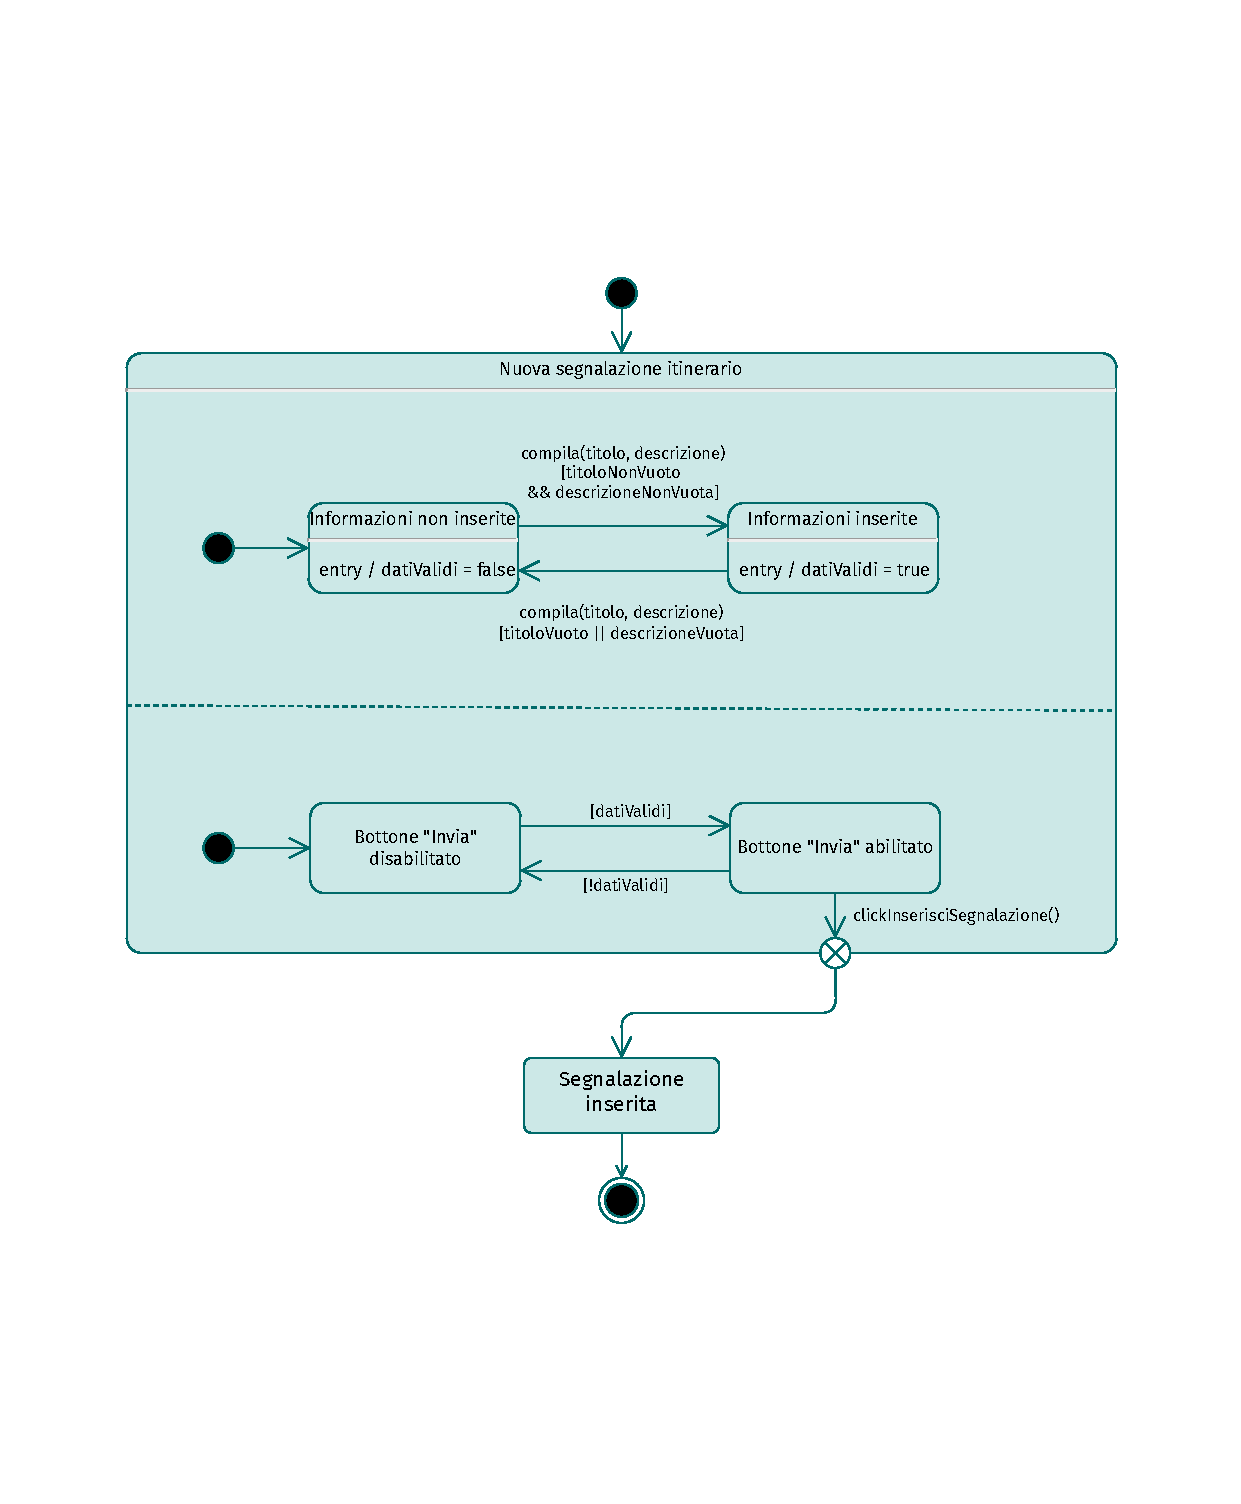
\includegraphics[width=\textwidth, page=1]{./diagrams/statechart.pdf}
	\caption{Nuova segnalazione itinerario}
\end{figure}
\FloatBarrier

\newpage
\subsubsection{Inserimento itinerario}
\begin{figure}[!htbp]
	\centering
	\includegraphics[width=\textwidth, page=2]{./diagrams/statechart.pdf}
	\caption{Nuovo itinerario}
\end{figure}
\FloatBarrier

\newpage
\subsubsection{Inserimento dettagli itinerario}
\begin{figure}[!htbp]
	\centering
	\includegraphics[width=\textwidth, page=3]{./diagrams/statechart.pdf}
	\caption{Regione interna - Inserimento dettagli itinerario}
\end{figure}
\FloatBarrier

\newpage
\subsubsection{Inserimento mappa itinerario}
\begin{figure}[!htbp]
	\centering
	\includegraphics[width=\textwidth, page=4]{./diagrams/statechart.pdf}
	\caption{Regione interna - Inserimento mappa itinerario}
\end{figure}
\FloatBarrier

\newpage
\subsubsection{Inserimento foto itinerario}
\begin{figure}[!htbp]
	\centering
	\includegraphics[width=\textwidth, page=5]{./diagrams/statechart.pdf}
	\caption{Regione interna - Inserimento foto itinerario}
\end{figure}
\FloatBarrier

\newpage
\subsection{Classi, oggetti e relazioni di analisi}

\newpage
\subsection{Diagrammi di sequenza di analisi}
Sono presentati nella seguente sezione i Sequence Diagram relativi a due funzionalità offerte dall'applicazione:
la segnalazione di un itinerario e la ricerca di un itinerario.
\\subsubsection{Segnalazione itinerario}
\begin{figure}[!htbp]
	\centering
	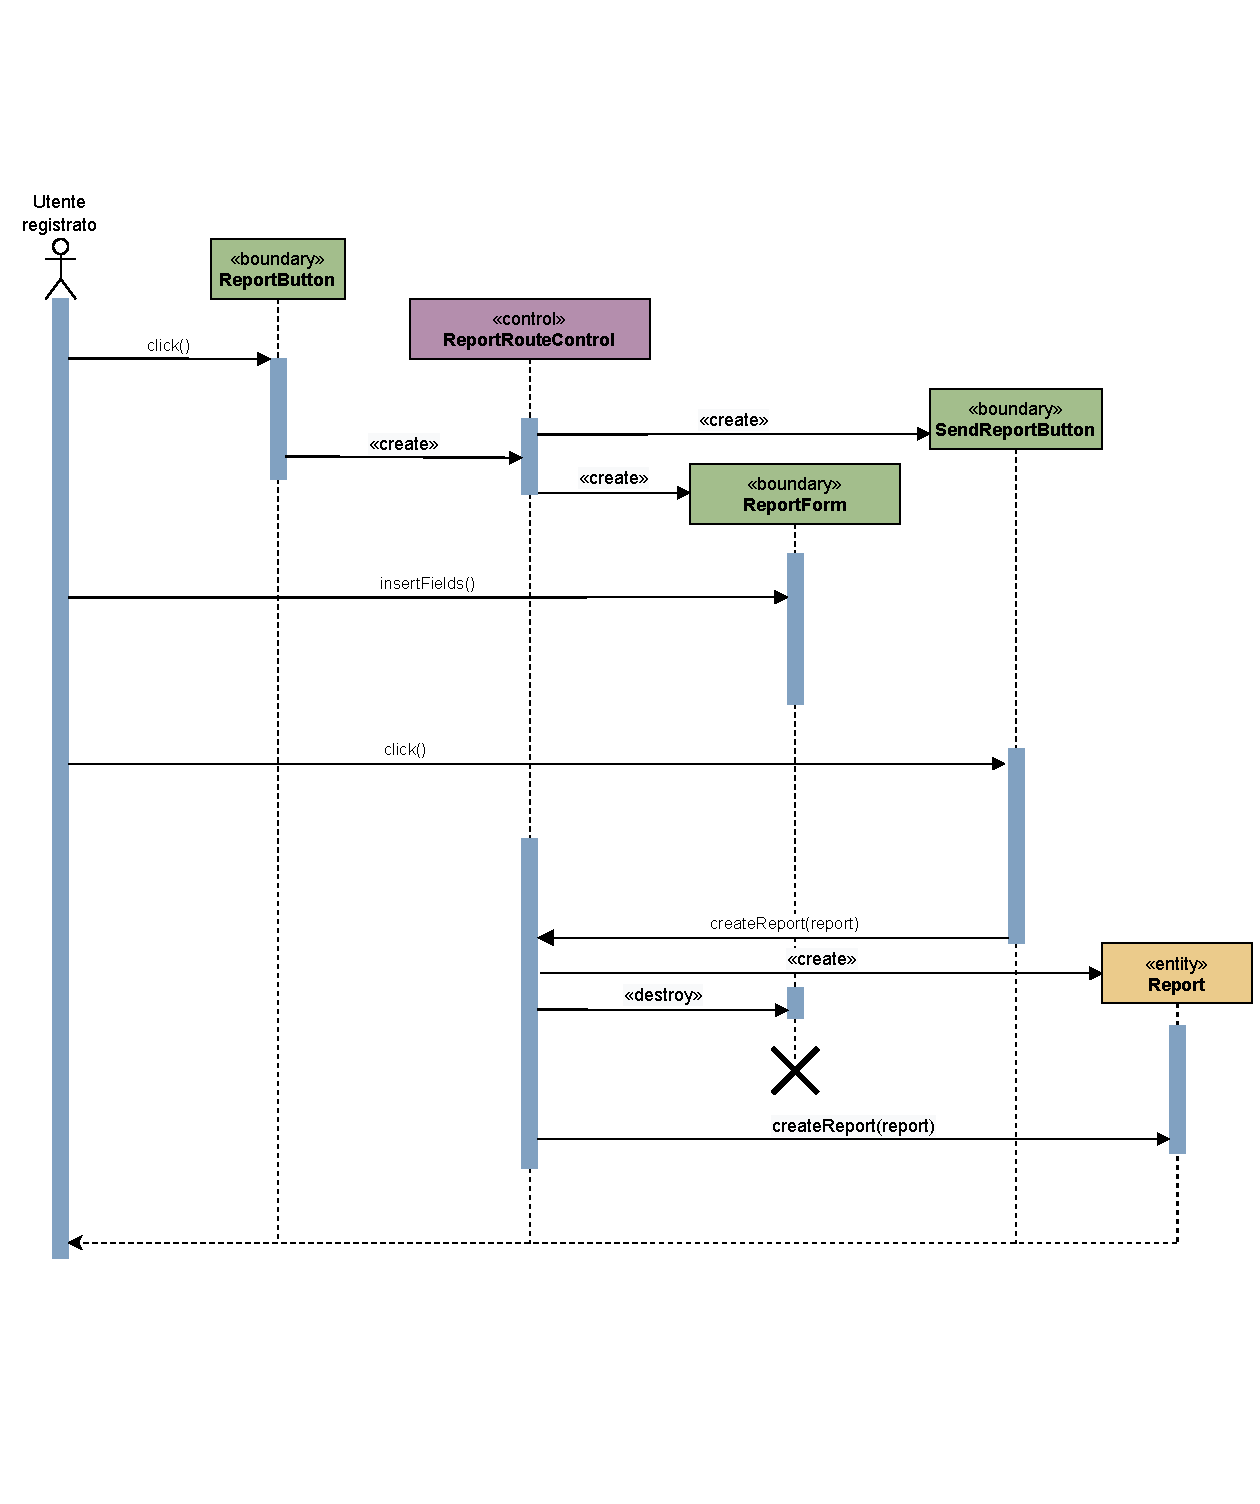
\includegraphics[width=\textwidth, page=1]{./diagrams/sequenceDomain-segnalazioneItinerario.pdf}
	\caption{Sequence Diagram 1 - Segnalazione di un itinerario}
\end{figure}
\FloatBarrier

\newpage
\subsubsection{Ricerca itinerario}
\begin{figure}[!htbp]
	\centering
	\includesvg[width=\textwidth, height=21cm]{./diagrams/sequenceDomain-ricercaItinerario.svg}
	\caption{Sequence Diagram 2 - Ricerca di un itinerario}
\end{figure}
\FloatBarrier

\newpage
\subsection{Diagrammi di attività}

\subsubsection{Autenticazione}
\begin{figure}[!htbp]
	\centering
	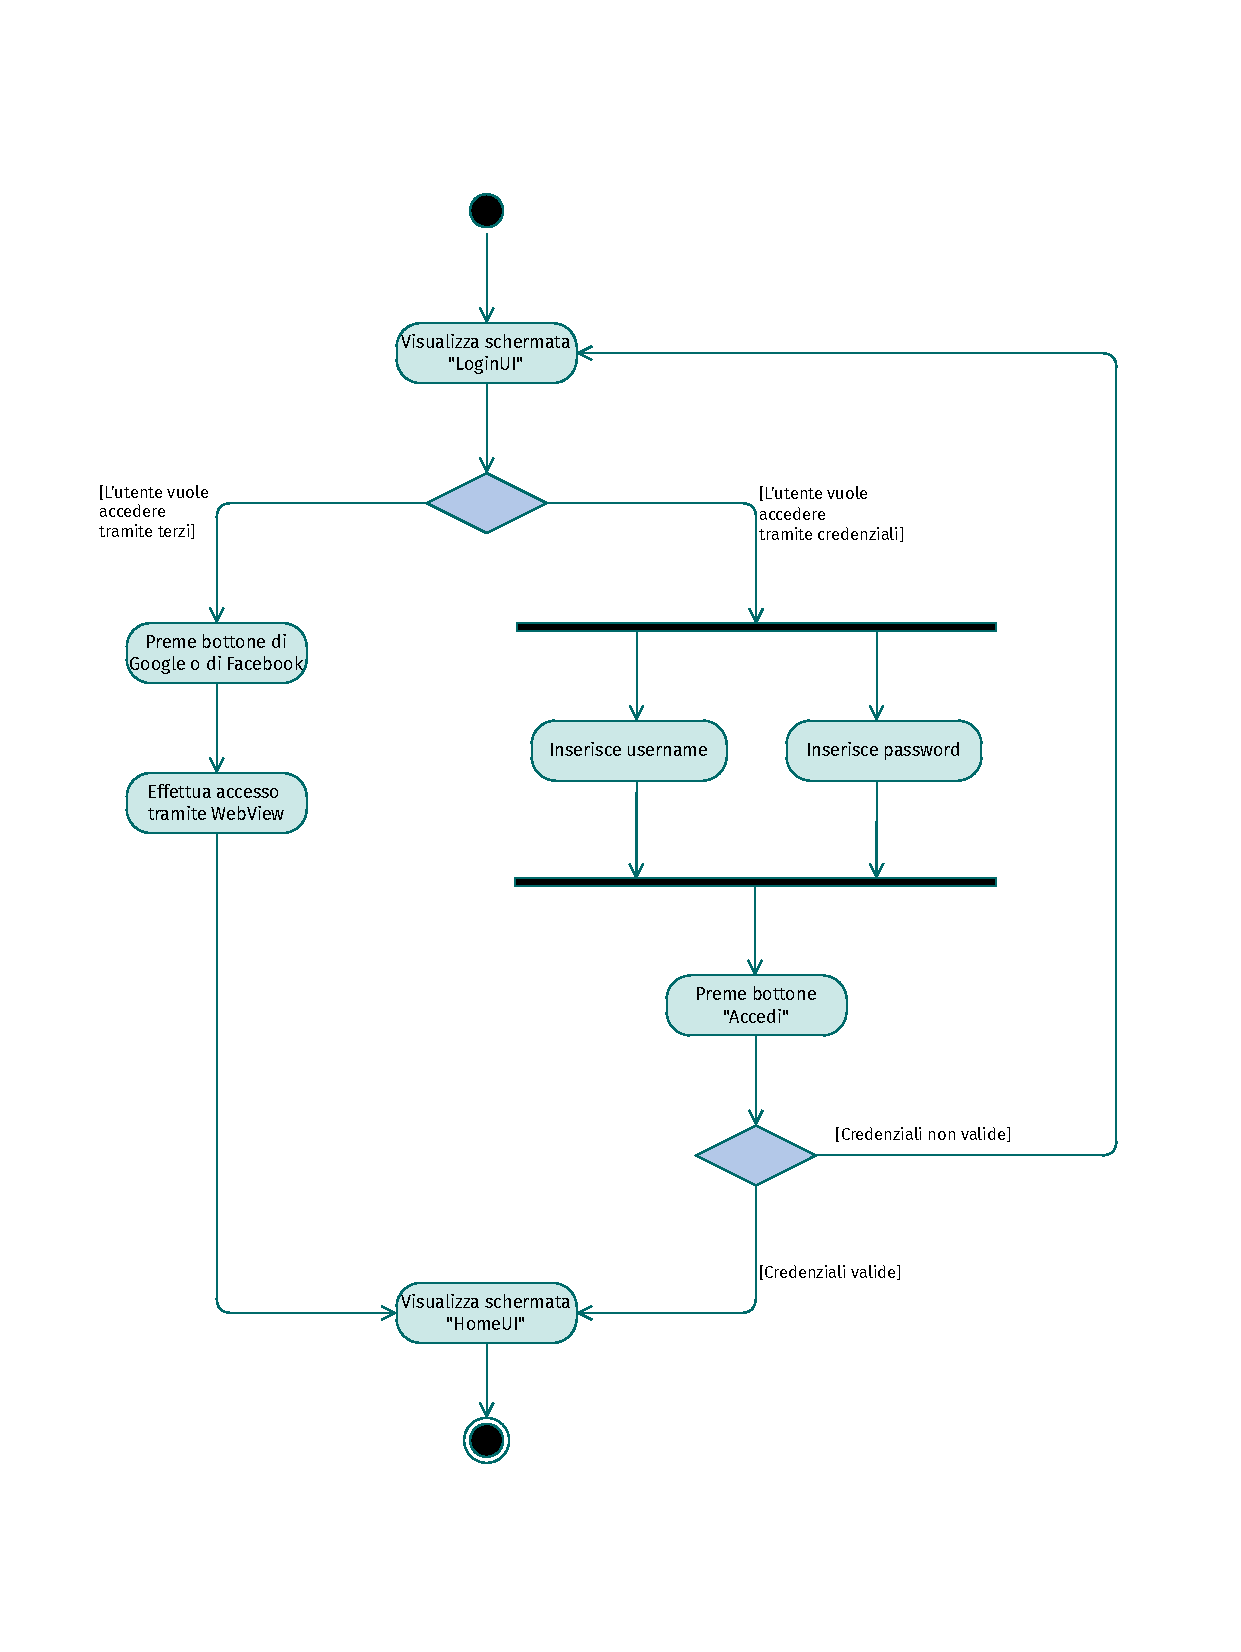
\includegraphics[width=\textwidth, page=1]{./diagrams/activity.pdf}
	\caption{Login utente}
\end{figure}
\FloatBarrier

\newpage
\begin{figure}[!htbp]
	\centering
	\includesvg[width=\textwidth, height=21cm]{./diagrams/activity-registrazione.svg}
	\caption{Registrazione utente}
\end{figure}
\FloatBarrier

\newpage
\begin{figure}[!htbp]
	\centering
	\includesvg[width=\textwidth, height=21cm]{./diagrams/activity-forgot_password.svg}
	\caption{Reset password dimenticata}
\end{figure}
\FloatBarrier

\newpage
\begin{figure}[!htbp]
	\centering
	\includegraphics[width=\textwidth, page=16]{./diagrams/activity.pdf}
	\caption{Logout}
\end{figure}
\FloatBarrier


\newpage
\subsubsection{Interazione con un itinerario}
\begin{figure}[!htbp]
	\centering
	\includesvg[width=\textwidth, height=21cm]{./diagrams/activity_aggiungi_itinerario.svg}
	\caption{Aggiunta itinerario}
\end{figure}
\FloatBarrier

\newpage
\begin{figure}[!htbp]
	\centering
	\includegraphics[width=\textwidth, page=9]{./diagrams/activity.pdf}
	\caption{Rimozione itinerario}
\end{figure}
\FloatBarrier

\newpage
\begin{figure}[!htbp]
	\centering
	\includegraphics[width=\textwidth, page=2]{./diagrams/activity.pdf}
	\caption{Ricerca itinerario}
\end{figure}
\FloatBarrier

\newpage
\begin{figure}[!htbp]
	\centering
	\includegraphics[width=\textwidth, page=10]{./diagrams/activity.pdf}
	\caption{Valutazione itinerario}
\end{figure}
\FloatBarrier

\newpage
\begin{figure}[!htbp]
	\centering
	\includegraphics[width=\textwidth, page=11]{./diagrams/activity.pdf}
	\caption{Salvataggio itinerario}
\end{figure}
\FloatBarrier

\newpage
\begin{figure}[!htbp]
	\centering
	\includegraphics[width=\textwidth, page=12]{./diagrams/activity.pdf}
	\caption{Segnalazione itinerario}
\end{figure}
\FloatBarrier

\newpage
\subsubsection{Interazione con un post}
\begin{figure}[!htbp]
	\centering
	\includegraphics[width=\textwidth, page=3]{./diagrams/activity.pdf}
	\caption{Aggiunta post}
\end{figure}
\FloatBarrier

\newpage
\begin{figure}[!htbp]
	\centering
	\includegraphics[width=\textwidth, page=4]{./diagrams/activity.pdf}
	\caption{Rimozione post}
\end{figure}
\FloatBarrier

\newpage
\begin{figure}[!htbp]
	\centering
	\includegraphics[width=\textwidth, page=14]{./diagrams/activity.pdf}
	\caption{Segnalazione post}
\end{figure}
\FloatBarrier

\newpage
\subsubsection{Interazione con una compilation}
\begin{figure}[!htbp]
	\centering
	\includegraphics[width=\textwidth, page=7]{./diagrams/activity.pdf}
	\caption{Aggiunta compilation}
\end{figure}
\FloatBarrier

\newpage
\begin{figure}[!htbp]
	\centering
	\includegraphics[width=\textwidth, page=9]{./diagrams/activity.pdf}
	\caption{Rimozione compilation}
\end{figure}
\FloatBarrier

\newpage
\begin{figure}[!htbp]
	\centering
	\includegraphics[width=\textwidth, page=8]{./diagrams/activity.pdf}
	\caption{Rimozione itinerario da compilation}
\end{figure}
\FloatBarrier

\newpage
\subsubsection{Gestione profilo e interazione con utenti}
\begin{figure}[!htbp]
	\centering
	\includegraphics[width=\textwidth, page=16]{./diagrams/activity.pdf}
	\caption{Invio messaggio}
\end{figure}
\FloatBarrier

\begin{figure}[!htbp]
	\centering
	\includegraphics[width=\textwidth, page=17]{./diagrams/activity.pdf}
	\caption{Ricerca destinatario messaggio}
\end{figure}
\FloatBarrier

\newpage
\begin{figure}[!htbp]
	\centering
	\includegraphics[width=\textwidth, page=15]{./diagrams/activity.pdf}
	\caption{Avvio conversazione con l'autore di un post o itinerario}
\end{figure}
\FloatBarrier

\newpage
\begin{figure}[!htbp]
	\centering
	\includegraphics[width=\textwidth, page=5]{./diagrams/activity.pdf}
	\caption{Modifica foto profilo}
\end{figure}
\FloatBarrier

\newpage
\subsubsection {Funzionalità riservate agli amministratori}
\begin{figure}[!htbp]
	\centering
	\includegraphics[width=\textwidth, page=18]{./diagrams/activity.pdf}
	\caption{Rimozione segnalazione}
\end{figure}
\FloatBarrier

\newpage
\begin{figure}[!htbp]
	\centering
	\includegraphics[width=\textwidth, page=19]{./diagrams/activity.pdf}
	\caption{Modifica itinerario}
\end{figure}
\FloatBarrier


\newpage
\section{Documento di Design del sistema}
\subsection{Analisi dell'architettura e criteri di design}
\subsubsection{Software deployment}
L'architettura del software realizzato pone le sue fondamenta nel concetto di \textbf{cloud computing}.\\
Il cloud computing, o computazione cloud, consiste nella distribuzione on-demand di risorse IT, con 
una tariffazione basata sul consumo.\\\\
Tra i diversi provider, è stato scelto di usufruire dei servizi offerti dalla piattaforma proprietaria del gruppo 
Amazon \textbf{AWS}, \textbf{Amazon Web Services}.
AWS offre infatti cloud services ideali per creare applicazioni in modo scalabile, flessibile e affidabile; esso 
presenta inoltre notevoli vantaggi, ritenuti come caratteristiche desiderabili per la progettazione di qualunque software.\\

La scelta della piattaforma AWS è stata compiuta, inoltre, per le seguenti qualità:
\begin{itemize}
	\item \textbf{Agilità} - la possibilità di aumentare a seconda delle necessità risorse quali servizi infrastrutturali, 
		  calcolo, storage e database;
	\item \textbf{Elasticità} - la possibilità di evitare l'allocazione anticipata di una quantità maggiore di risorse di 
			quante siano necessarie, così da gestire i picchi nei livelli di attività future;
	\item \textbf{Distribuzione globale di contenuti} - l'infrastruttura AWS offre una copertura globale: fare in modo che le 
		  applicazioni siano vicino agli utenti finali riduce la latenza e migliora la loro esperienza.\\
\end{itemize}


AWS offre una grande varietà di servizi; ciascuno di essi va incontro a una specifica necessità dello sviluppatore. \\
Nello sviluppo del software, per implementare determinate funzionalità si è scelto di ricorrere all'utilizzo dei seguenti servizi:
\begin{itemize}
	\item \textbf{Cognito} - Amazon Cognito permette di aggiungere strumenti di registrazione degli utenti, accesso 
		  e controllo degli accessi alle app Web e per dispositivi mobili. Esso supporta l'accesso degli utenti 
		  tramite l'uso di provider di identità social quali Facebook, Google. 
		  Tale risorsa è stata sfruttata realtivamente all'autenticazione utente, tenendo particolarmente in considerazione 
		  l'alto fattore di sicurezza che essa conferisce;
	\item \textbf{EC2} - l'\textbf{Elastic Compute Cloud} (Amazon EC2) fornisce capacità di calcolo scalabile in AWS Cloud. 
		  Esso offre ambienti di elaborazione virtuale, noti come \textit{istanze}, varie configurazioni di CPU, memoria, 
		  archiviazione e capacità di rete per le istanza note come \textit{tipi di istanza}. 
		  La scelta di tale servizio è stata finalizzata al deploy dell'applicativo Spring, nella realizzazione del Rest Service.
	\item \textbf{RDS} - Amazon RDS ha permesso la configurazione e l'utilizzo del database relazionale alla base del software prodotto;
	\item \textbf{S3} - il \textbf{Simple Storage Service} (Amazon S3) permette l'archiviazione di oggetti in modo scalabile. 
		  Esso è stato adoperato in merito alla preservazione permanente dei file immagine caricati dagli utenti;
	\item \textbf{Lambda} - AWS Lambda è un servizio di calcolo basato su eventi serverless. 
		  La scelta del servizio Lambda è stata incentivata dalla sua possibilità di integrazione con il servizio \textbf{Cognito}, e dettata 
		  dalla volontà di conferire \textit{consistenza} al pool utenti del sistema.
		  Nello specifico, si è sfruttata la possibilità offerta dal servizio di creare dei \textit{trigger} (in particolare trigger di \textit{post conferma}), al fine di 
		  evitare - in seguito al processo di registrazione - la possibile presenza di inconsistenze tra database e registrazioni effettivamente portate a termine.
\end{itemize}

Si è ritenuto inoltre fondamentale l'utilizzo del framework \textbf{Amplify}.\\
In particolare, Amplify è stato impiegato per realizzare:
\begin{itemize} 
	\item Un servizio di autenticazione particolarmente sicuro tramite, come citato, il servizio \textit{Cognito};
	\item L'archiviazione di file (nella prima versione del software solo di file immagine) tramite il servizio \textit{S3}.
\end{itemize}

È importante specificare che il framework Amplify consente anche di creare back-end o applicativi serverless. Ciononostante, si sottolinea che 
nella realizzazione del software è stata fatta la scelta di utilizzarlo \textit{solo} in funzione dei servizi da essi offerti, soprattutto in relazione alla deprecazione 
dell'SDK standard AWS per Android.

\subsubsection{Google Maps Platform}
Una delle caratteristiche principali del software risulta essere la forte componente geolocalizzata degli itinerari presenti in piattaforma. \\
Gli utenti, infatti, nell'inserimento e nella visualizzazione dei sentieri si trovano ad interfacciarsi direttamente con mappe interattive.
Per garantire un'esperienza ottimale da questo punto di vista sono stati utilizzati i servizi della piattaforma Google Maps. \\\\
La \textbf{Google Maps Platform} è un insieme di API e SDK che permette di integrare in applicazioni mobile Google Maps, e di recuperare dati da esso stesso.
L'esperienza utente con le funzionalità sopracitate è stata supportata dall'utilizzo delle seguenti API:
\begin{itemize}
	\item MapsAPI - per la visualizzazione interattiva di mappe statiche e dinamiche;
	\item PlacesAPI - per il recupero di informazioni sui posti tramite richieste HTTP;
	\item DirectionsAPI - per il calcolo del percorso tra diverse tappe; utilizzano una richiesta HTTP per ritornare le direzioni tra località in formato JSON o XML. 
		  Le DirectionsAPI, in quanto web service, sono state integrate nel Rest Service proprio del software.
\end{itemize}

\subsubsection{Architettura del Rest Service}
Nella realizzazione del Rest Service è stato scelto di utilizzare il framework \textbf{Spring}. \\
Spring fornisce un'\textit{infrastruttura di supporto} per lo sviluppo di applicazioni: esso prevede una \textit{modularizzazione} dell'architettura come segue:
\begin {itemize}
	\item Presentation layer - strato più esterno, che gestisce la presentazione del contenuto e l'interazione con l'utente;
	\item Business logic layer - strato centrale, che gestisce la logica;
	\item Data access layer - strato più interno, che gestisce il recupero di dati dalle diverse sorgenti.
\end{itemize}

Ciascuno di questi strati dipende da quello sottostante per far sì che l'applicazione funzioni. In altre parole,
lo strato di presentazione comunica con quello della business logic, che a sua volta comunica con lo strato di data 
access. Ogni strato ha quindi bisogno di questa \textit{dipendenza} per eseguire il proprio compito correttamente \\

La scelta di utilizzare il framework Spring è stata fatta in relazione alla volontà di ottenere un \textit{loose coupling}, ossia un accoppiamento largo. 
Senza l'utilizzo di Spring, ci sarebbe stata la possibilità che il codice avesse potuto causare \textit{tight coupling}, che non è 
considerato essere una buona pratica di programmazione. Il loose coupling è ideale, in quanto le componenti largamente 
accoppiate sono indipendenti: ciò implica che, a seguito di possibili cambiamenti futuri, questi non influenzeranno 
le altre componenti.\\

Al cuore del framework Spring si trova la \textbf{dependency injection}. \\
La dependency injection è un pattern di programmazione che permette agli sviluppatori di costruire architetture disaccoppiate. Ciò vuol dire che Spring comprende le \textit{annotazioni} 
poste in capo alle classi; in seguito alla creazione di un'istanza, dunque, il framework si assicura che le istanze siano state create con le opportune dependencies. \\\

Nello specifico, per l'implementazione del software, è stata utilizzata un'estensione del framework Spring, chiamata \textbf{Spring Boot}.\\
Spring Boot ha delle caratteristiche specifiche che rendono la gestione dell'applicazione più semplice.\\
Tra alcuni dei vantaggi che hanno portato alla scelta di Spring Boot, si ricordano:
\begin{itemize}
	\item Creazione di applicazioni Spring stand-alone;
	\item Dotazione di dependencies "starter" per semplificare la configurazione di build;
	\item Configurazione automatica di Spring e di librerie di terze parti, ove possibile;
	\item Nessuna generazione di codice e nessun requisito per la configurazione XML;
	\item Inclusione di un web server embedded (nello specifico \textit{Apache Tomcat}) senza la necessità di ulteriori configurazioni.
\end{itemize}

\newpage
\subsection{Architettura dell’applicativo}
L'intera architettura del software è stata progettata seguendo le linee guida della cosiddetta \textbf{Clean Architecture}. \\
Il concetto di architettura \textit{pulita} si basa sui principi enunciati da Robert C. Martin nel libro "Clean Architecture".
In seguito alle informazioni acquisite dalla lettura del libro, infatti, questo approccio è stato ritenuto quello più valido.\\
L’idea chiave è quella di utilizzare il principio di inversione di dipendenza per porre dei boundaries tra componenti di alto livello e componenti di basso livello. 
Ciò crea un’architettura \textit{plug-in}, 
che conferisce al sistema un’elevata flessibilità e un'elevata manutenibilità. \\
Un’architettura \textit{pulita} inizia da un codice \textit{pulito}. Classi pulite derivano da componenti pulite, che, a loro volta, determinano un \textit{sistema pulito}.\\
È stato quindi ritenuto di fondamentale importanza applicare i principi della Clean Architecture e del Clean Code in maniera uniforme e costante, nell'implementazione di qualsiasi componente.\\

Il concetto di \textit{Clean Code} sfruttato nello sviluppo del software segue i principi \textbf{SOLID}. \\ 
Tali principi sono stati applicati in modo da ottimizzare l’architettura e ciascuna delle sue componenti, le quali risultano dunque essere caratterizzate dal:
\begin{itemize}
	\item \textbf{Single responsability principle} – una classe dovrebbe avere uno ed un solo motivo per cambiare;
	\item \textbf{Open-closed principle} – una classe dovrebbe essere aperta all’estensione ma chiusa alle modifiche;
	\item \textbf{Liskov’s substitution principle} – gli oggetti di un programma dovrebbero essere sostituibili con istanze dei propri sottotipi senza alterare la correttezza del programma stesso;
	\item \textbf{Interface segregation principle} – più interfacce client-spefic sono meglio di un’unica interfaccia general-purpose;
	\item \textbf{Dependency inversion principle}\footnote{
	Il principio di inversione di dipendenza è stato applicato, in particolare, in relazione agli UseCase (nel Domain Layer): la loro indipendenza dagli altri moduli fa in modo che essi possano dipendere 
	solo da \textit{astrazioni} dei loro strati.} 
	– i moduli di alto livello non dovrebbero dipendere da moduli di basso livello; entrambi dovrebbero dipendere da \textit{astrazioni}.
\end{itemize}

Il concetto di Clean Architecture si basa sulla \textit{modularità} dell’architettura stessa. \\
Nel caso della progettazione del software prodotto è stata seguita una suddivisione del seguente tipo:
\begin{itemize}
	\item Presentation layer – responsabile della presentazione a schermo e della gestione delle 
		interazioni degli utenti;
	\item Domain layer – rappresentazione formale del dominio applicativo
	\item Data layer – contenitore delle implementazioni delle sorgenti di dati e dei repository, 
		i quali coordinano i dati provenienti da esse.
\end{itemize}

È bene sottolineare, però, che nell'effettiva implementazione dell'applicativo non è
stato pedissequamente seguito lo schema appena proposto. \\ 
È stato ritenuto più opportuno adottare un approccio \textit{per funzionalità}; ciò è risultato nell'applicazione del concetto di \textbf{Screaming Architecture.} \\
L'espressione "Screaming Architecture" è stata coniata dal sopracitato Robert C. Martin; essa viene utilizzata nelle situazioni in cui, 
rivolgendo un solo sguardo ad un progetto, si riesce ad avere un'idea di base su cosa esso faccia e su cosa riguardi. \\
Da ciò deriva la possibilità di comprendere esattamente la struttura al cuore del codice implementato: 
la suddivisione nei diversi package "urla" al lettore l'approccio utilizzato, che risulta dunque chiaro e compresibile già a primo impatto.\\

La Clean Architecture non preclude, però, la possibilità di adattare all'applicativo un proprio design pattern architetturale. \\
Come descritto nella sezione successiva, tale approccio è stato ritenuto adatto alle esigenze di implementazione.

\newpage
\subsubsection{Pattern architetturali}
Quest'ultima potrebbe infatti essere definita come \textit{ibrida}: ciò è dovuto alla 
\textit{fusione} di due pattern architetturali differenti utilizzati nella progettazione. \\
Tali pattern sono \textbf{MVVM} e \textbf{MVI}; quest'ultimo è stato utilizzato per ovviare ai problemi 
sofferti dal primo. Procediamo ad un'analisi più dettagliata. \\

\textbf{MVVM} è un'architettura del tipo Model-View-ViewModel che evita l'accoppiamento stretto 
tra ciascuna componente. Più nello specifico, in questo tipo di architettura, i figli non hanno un 
riferimento diiretto al padre, ma hanno solo riferimenti tramite \textit{observables}.\\
Esso è organizzato secondo tre strati:
\begin{itemize}
	\item Model - rappresenta i dati e la business logic dell'applicazione;
	\item View - consiste del codice relativo alle interfacce utente;
	\item ViewModel - definisce una sorta di ponte tra i due modelli sopracitati.
\end{itemize}

Il modello MVVM, per quanto affermato, pone però alcune problematiche, quali ad esempio 
la difficoltà di riusabilità sia per le views che per i view model, la complicata comunicazione tra le 
componenti ecc. \\

A questo scopo, è stata realizzata un'integrazione con il modello MVI. \\

\textbf{MVI} sta per Model-View-Intent. Si tratta di uno dei pattern architetturali più nuovi per applicazioni Android. 
\begin{itemize}
	\item Model - rappresenta uno stato. I model dovrebbero essere immutabili, in modo da 
		  assicurare un flow di dati unidirezionale con gli altri strati;
	\item View - rappresenta le view, che possono essere implementati in activity o fragment
	\item Intent - rappresenta un'intenzione o una volontà di eseguire un'azione, sia dell'utente 
		  che dell'app stessa.
\end{itemize}


\newpage
\subsubsection{Diagramma di design del sistema}
\begin{figure}[!htbp]
	\centering
	 \includepdf[pages=1]{./diagrams/sysdesign.pdf}
\end{figure}

\newpage
\subsection{Diagramma delle classi di design}

\subsubsection{Autenticazione}
\begin{figure}[!htbp]
	\centering
	\includesvg[width=\textwidth, height=21cm]{./diagrams/design/login.svg}
	\caption{Login e Login con social}
\end{figure}

\newpage
\subsubsection{Interazione con una compilation}
\begin{figure}[!htbp]
	\centering
	\includesvg[width=\textwidth, height=21cm]{./diagrams/design/dettaglio_itinerario.svg}
	\caption{Dettaglio compilation e rimozione itinerario da compilation}
\end{figure}

\newpage
\subsubsection{Aggiunta di un itinerario}
\begin{figure}[!htbp]
	\centering
	\includesvg[width=\textwidth, height=21cm]{./diagrams/design/design_class_diagrams-Crea_itinerario}
	\caption{Aggiunta di un nuovo itinerario}
\end{figure}



\newpage
\subsection{Diagrammi di sequenza di design}
Sono di seguito presentati i diagrammi di sequenza di design per due casi d'uso significativi.

\newpage
\subsection{Definizione delle gerarchie funzionali}

\newpage
\section{Definizione di un piano di testing e valutazione sul campo dell'usabilità}


\end{document}